\documentclass[11pt]{article}
\usepackage{cite}

\usepackage{hyperref}
%biblio
\usepackage{natbib}
\usepackage{url}
\usepackage{wrapfig}

%Math
\usepackage{amsmath}
\usepackage{amsfonts}
\usepackage{amssymb}
\usepackage{amsthm}
\usepackage{ulem}
\usepackage{stmaryrd} %f\UTF{00FC}r Blitz!

%PageStyle
%\usepackage[ngerman]{babel} % deutsche Silbentrennung1
\usepackage[utf8x]{inputenc} 
\usepackage{fancyhdr, graphicx}
\usepackage{subcaption}
\usepackage[scaled=0.92]{helvet}
\usepackage{enumitem}
\usepackage{parskip}
\usepackage[a4paper,top=2cm]{geometry}
\setlength{\textwidth}{17cm}
\setlength{\oddsidemargin}{-0.5cm}
\usepackage{lastpage} % for getting last page number
\renewcommand{\familydefault}{\sfdefault}
\usepackage{setspace}
\usepackage{acronym}


% Code listenings
\usepackage{color}
\usepackage{xcolor}
\usepackage{listings}
\usepackage[font=it]{caption}
\DeclareCaptionFont{white}{\color{white}}
\DeclareCaptionFormat{listing}{\colorbox{gray}{\parbox{\textwidth}{#1#2#3}}}
\captionsetup[lstlisting]{format=listing,labelfont=white,textfont=white}
\lstset{
 language=Java,
 basicstyle=\footnotesize\ttfamily, % Standardschrift
 numbers=left,               % Ort der Zeilennummern
 numberstyle=\tiny,          % Stil der Zeilennummern
 stepnumber=5,              % Abstand zwischen den Zeilennummern
 numbersep=5pt,              % Abstand der Nummern zum Text
 tabsize=2,                  % Groesse von Tabs
 extendedchars=true,         %
 breaklines=true,            % Zeilen werden Umgebrochen
 frame=b,         
 %commentstyle=\itshape\color{LightLime}, Was isch das? O_o
 %keywordstyle=\bfseries\color{DarkPurple}, und das O_o
 basicstyle=\small,
 stringstyle=\color[RGB]{42,0,255}\ttfamily, % Farbe der String
 keywordstyle=\color[RGB]{127,0,85}\ttfamily, % Farbe der Keywords
 commentstyle=\color[RGB]{63,127,95}\ttfamily, % Farbe des Kommentars
 showspaces=false,           % Leerzeichen anzeigen ?
 showtabs=false,             % Tabs anzeigen ?
 xleftmargin=17pt,
 framexleftmargin=17pt,
 framexrightmargin=5pt,
 framexbottommargin=4pt,
 showstringspaces=false      % Leerzeichen in Strings anzeigen ?        
}

%Config
\fancypagestyle{firststyle}{ %Style of the first page
 \fancyhf{}
 \fancyheadoffset[L]{0.6cm}
 \lhead{
 
\includegraphics[scale=0.8]{./fhnw_ht_e_10mm.jpg}}
 \renewcommand{\headrulewidth}{0pt}
 \lfoot{Institute 4 Data Science,\linebreak www.fhnw.ch }
}

\fancypagestyle{documentstyle}{ %Style of the rest of the document
 \fancyhf{}
 \fancyheadoffset[L]{0.6cm}
\lhead{
 
\includegraphics[scale=0.8]{./fhnw_ht_e_10mm.jpg}}
 \renewcommand{\headrulewidth}{0pt}
 \lfoot{P7 Compressed Sensing Image Reconstruction for CASA}
 \rfoot{\thepage\ / \pageref{LastPage} }
}

\fancypagestyle{tableofcontent}{ %Style of the rest of the document
 \fancyhf{}
 \fancyheadoffset[L]{0.6cm}
\lhead{
 
\includegraphics[scale=0.8]{./fhnw_ht_e_10mm.jpg}}
 \renewcommand{\headrulewidth}{0pt}
 \cfoot{\thepage}
}

\fancypagestyle{abstract}{ %Style of the first page
 \fancyhf{}
 \fancyheadoffset[L]{0.6cm}
 \lhead{
 
\includegraphics[scale=0.8]{./fhnw_ht_e_10mm.jpg}}
 \renewcommand{\headrulewidth}{0pt}
 \cfoot{}
}


%Metadata
\numberwithin{equation}{section}


\begin{document}
\title{P7 Compressed Sensing Image Reconstruction for CASA}
\author{Jonas Schwammberger}
\date{\today}
\maketitle

\newpage
\pagestyle{abstract}
\section*{Abstract}
The MeerKAT new Radio Interferometer poses an image reconstruction problem on a large scale. Measurements over terabytes in size should be reconstructed to an image. Compressed Sensing reconstructions have the potential to improve the effective accuracy of MeerKAT, but so far were more expensive than the state of the art CLEAN implementation.

current Compressed Sensing approaches use the non-uniform FFT to cycle between Visibility and image space. But compared to CLEAN, they need more cycles to converge, which is one reason why Compressed Sensing reconstructions have higher runtime costs.

Creating a scalable image reconstruction algorithm for MeerKAT is still an open problem.

In this project, we postulated that by replacing the non-uniform FFT approximation, we might get a Compressed Sensing algorithm with lower runtime costs.

In the large scale MeerKAT problems, calulating the Fourier Transform becomes an issue. Current Compressed Sensing implementations and CLEAN use the non-uniform FFT approximation, which leads to a similar architecture. In this work, we discuss three alternatives to the non-uniform FFT. We created a new algorithm which uses the direct Fourier Transform and Coordinate Descent. It does not need the approximation and naturally extends to wide field of view measurements of MeerKAT. Our algorithm leverages the starlet transform and only needs to calculate the transform for non-zero bases. This leads to a reconstruction algorithm, which scales with the number of non-zero components.

We compare our Coordinate Descent algorithm to CLEAN on simulated MeerKAT data. WE show the superior reconstruction quality and extrapolate the runtime costs of our approach to a real-world MeerKAT observation. Sadly, our algorithm could not improve the runtime costs compared to CLEAN. Coordinate Descent has interesting properties for distribution, but in the current state our algorithm is too expensive to be competitive.

We postulate that there is no single a

%TOC
\newpage
\pagestyle{tableofcontent}
\pagenumbering{Roman}
\tableofcontents  	
\newpage

\pagestyle{documentstyle}
\setcounter{page}{1}
\pagenumbering{arabic}

\section{Compressed Sensing Image Reconstruction for MeerKAT} \label{intro}
An instrument in the real world measures noisy data. Measurements are corrupted by noise, interference sources or the measurement instrument itself. Image reconstruction problems appear when one tries to remove the corruption from the measurements and tries to find the observed image of the instrument. This leads to an ill-posed inverse problem: A small change in the measurements may create very different image reconstructions, and many possible images match the measurements. An image reconstruction algorithm therefore has to find the observed image from a potentially large set of possible images.

In the past, image reconstructions applied simple heuristics and approximated a likely image. How close the approximation was to the observed image was in general not known. The theory of compressed sensing\cite{candes2006robust}\cite{donoho2006compressed} introduced a new theoretical framework under which image reconstructions can be analysed. This has lead rise to new compressed sensing reconstruction algorithms, which under the right conditions are guaranteed to reconstruct the observed image. Furthermore they have shown super-resolution performance in real-world environments, creating reconstructions above the accuracy limit of the instrument.

This work applies compressed sensing image reconstruction to the field of radio astronomy. The new MeerKAT radio interferometer poses a reconstruction problem on a new scale of data volume. The raw measurements easily take up several terabytes of disk space. The focus of this work is creating a scalable compressed sensing image reconstruction algorithm.

The current state of the art reconstruction algorithm for MeerKAT is based on CLEAN\cite{rich2008multi}\cite{rau2011multi}. It is a reconstruction using a simple heuristic and was developed before the theory of compressed sensing was known. In recent years, compressed sensing reconstruction algorithms were developed for radio interferometers\cite{girard2015sparse}\cite{dabbech2018cygnus}\cite{birdi2018sparse}. They beat CLEAN in terms of reconstruction quality, producing super-resolved reconstructions. However, CLEAN has the upper hand in runtime complexity. Therefore, an efficient implementation of CLEAN is still the go to reconstruction algorithm for MeerKAT data.

The efficient implementation use CLEAN in the Major Cycle Architecture, which was developed with CLEAN in mind. Current compressed sensing algorithms use a similar architecture. So far, little research has gone into different architectures for compressed sensing reconstructions in radio astronomy. This work explores different architectures for compressed sensing reconstructions with the hope of reducing the computational complexity. 

A new proof-of-concept reconstruction algorithm was developed with a simplified architecture. It was tested on simulated MeerKAT data and the lower-bound asymptotic complexity was evaluated. The new algorithm scales independently of the image size, but scales worse with the number of input measurements compared to CLEAN. For the MeerKAT image reconstruction, the number of input measurements tends to be the largest of all numbers in the problem. Even though the algorithm could be improved further, it is unlikely to beat CLEAN reconstructions in terms of runtime complexity on MeerKAT data.

%something something measurement equation

\subsection{The basic Measurement Equation of a radio interferometry}\label{intro:basic}
Real world radio interferometers have complicated measurement equations. They become even more complicated for large interferometers like MeerKAT. These problems get addressed in section \ref{meerkat}. This section looks at the basic measurement equation of a radio interferometer \eqref{intro:measurement} and discusses the two fundamental challenges for radio interferometry image reconstruction. 

\begin{equation}\label{intro:measurement}
V(u, v) = \int\int I(x, y) e^{2 \pi i (ux+vy)} \: dx \: dy
\end{equation}

An interferometer measures Fourier Components $V$ (called Visibilities in Radio Astronomy) from the sky image $I$ at position $x$ and $y$. The term $e^{2 \pi i (ux+vy)}$ represents the two dimensional Fourier Transform. The task is to reconstruct the observed image $I$ from the measured Visibilities $V$. In theory this task is trivial: Since the inverse Fourier Transform exists, we can reconstruct the image $I$ by calculating the inverse Fourier Transform of $V$. However, two properties of the Visibilities make this task challenging in practice:

\begin{enumerate}
	\item Non-uniform sampling pattern in Visibility space
	\item Incomplete Visibility coverage. 
\end{enumerate} 

\textit{Property 1:} We want to reconstruct an image with uniformly spaced pixels. The instrument defines the sampling pattern in Visibility space and does not correspond to the exact pixels of the reconstructed image. This property keeps us from using the Fast Fourier Transform. The naive inverse Fourier Transform can still be calculated, but it has a quadratic runtime and does not scale to the data volume of interferometers. Current reconstruction algorithms use the non-uniform Fast Fourier Transform. The non-uniform FFT approximates the non-uniform Fourier Transform. 

\textit{Property 2:} Interferometers sample only a limited set of Visibilities. It does not have all information for reconstruction. When the inverse Fourier Transform is applied on the Visibilities, the resulting image is corrupted by the incomplete Visibilities. It contains structures which where introduced by the interferometer and were not observed. With only knowing the incomplete set of Visibilities a reconstruction algorithm has to decide which image structures were truly measured, and which are due to the instrument. This forms an ill-posed inverse problem. There are many images that fit the measurements, and a small change in the Visibilities can lead to a very different reconstruction. 

CLEAN represents the instrumental effect with a Point Spread Function (PSF). After the non-uniform FFT produced the 'dirty' image, CLEAN tries to reconstruct observed image with a deconvolving the 'dirty' image with the PSF. Note however that both CLEAN nor the non-uniform FFT are approximations. In real world reconstructions, these two approximations are used in the major cycle architecture to increase the reconstruction accuracy. 

%The CLEAN algorithms approximate the observed image with a deconvolution: The inverse Fourier Transform produces a corrupted image. The observed image was convolved with a known Point Spread Function (PSF), which represents the instrument corruption. Finding a deconvolution reconstructs the observed image. The deconvolution is still an ill-posed problem, there are potentially many possible deconvolutions, and a small change in the input can lead to a very different output. Furthermore the CLEAN algorithms produce a greedy approximation of the deconvolution. 


\subsection{The Major Cycle Architecture}
Major cycle was created with CLEAN in mind. Compressed sensing reconstructions use essentially the same architecture with minor modifications. 

A CLEAN image reconstruction for radio interferometers consists of two different steps: A non-uniform FFT, which approximates the inverse Fourier Transform efficiently and an deconvolution algorithm, which approximates the instrumental effects on the image (typically based on CLEAN). These two approximations are an error source of the reconstruction. The major cycle architecture \ref{intro:major} therefore tries to iteratively minimize the errors of the non-uniform FFT and the deconvolution over several iterations.

\begin{wrapfigure}{r}{0.6\textwidth}
	\centering
	\vspace{-10pt}
	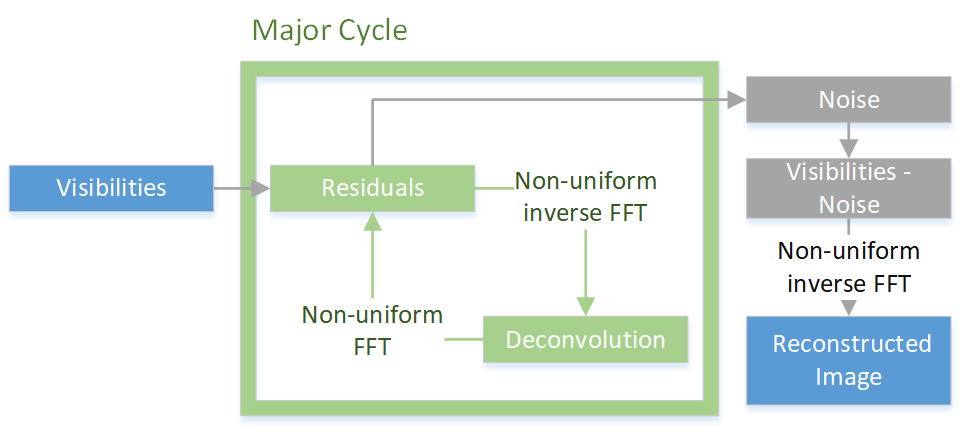
\includegraphics[width=1.0\linewidth]{./chapters/01.intro/Major-Minor.png}
	\caption{The Major Cycle Framework}
	\label{intro:major}
	\vspace{-10pt}
\end{wrapfigure}

The first major cycle uses the non-uniform inverse FFT to approximate the 'dirty' image from the Visibilities. The deconvolution algorithm decides parts which parts belong to the observed image and which are due to instrumental and other noise effects. It returns the noise part of the image, which gets transformed back into residual Visibilities. The next major cycle iteration continues with the residual Visibilities. The residual Visibilities get minimized until they contain only the instrumental effects and noise.

After several major cycles the residual  on a regularly spaced image which has a small error from non-uniform samples, and a small error from incomplete measurements.

Compressed sensing reconstructions essentially use the same architecture, although with minor alterations. In general, they keep a similar scheme of forward/backward non-uniform FFT, but do not use a deconvolution in image pace. Instead, they analyse constraints defined on the image (For example all pixels should be non-negative), and try to find the Visibilities that minimize the constraint violations.

For CLEAN reconstructions, the forward/backward non-uniform FFT are the most expensive operations, while the deconvolution is negligible. The compressed sensing algorithms tend to require more major cycle iterations to converge and the image constraint analysis tends to be more expensive than CLEAN deconvolutions. Current research into compressed sensing reconstructions is focussed on reducing the number of major cycles\cite{dabbech2018cygnus}. 

%Different architecture, but has to somehow handle all the difficulties that arise from imaging meerkat data.


%compressed sensing got rid of the miinor cycle, but essentially kept the major cycle framework
%have to handle own problems in a new architecture







\newpage
\section{Challenges for imaging MeerKAT data} \label{meerkat}

There are several challenger for imaging meerkat data. One problem is the new amount of data.

terabytes of measurements. Large image size 32k squared are the obvious problems to solve. Distributing the problem is not part of this work.

 In this work, it is focused on Wide field of view issue. 


Self calibration Calibration gets not explicitly called, but 

Further issues that do not get handled here
\begin{itemize}
	\item (Beam Pattern, A Projection)
	\item Full polarization
	\item Wide band imaging
\end{itemize}



\subsection{Wide Field of View Imaging} \label{wof}
W-Projection images 

Small field of view


But actually, there is a third component of the measurement equation \eqref{intro:measurement}

\begin{equation}\label{meerkat:ftsphere}
V(u, v, w) = \int\int \frac{X(x, y)}{\sqrt{1 - x^2 - y ^2}} e^{2 \pi i (ux+vy+ w\sqrt{1 - x^2 - y ^2})}dx dy
\end{equation}


\begin{figure}[h]
	\centering
	\begin{subfigure}[b]{0.45\linewidth}
		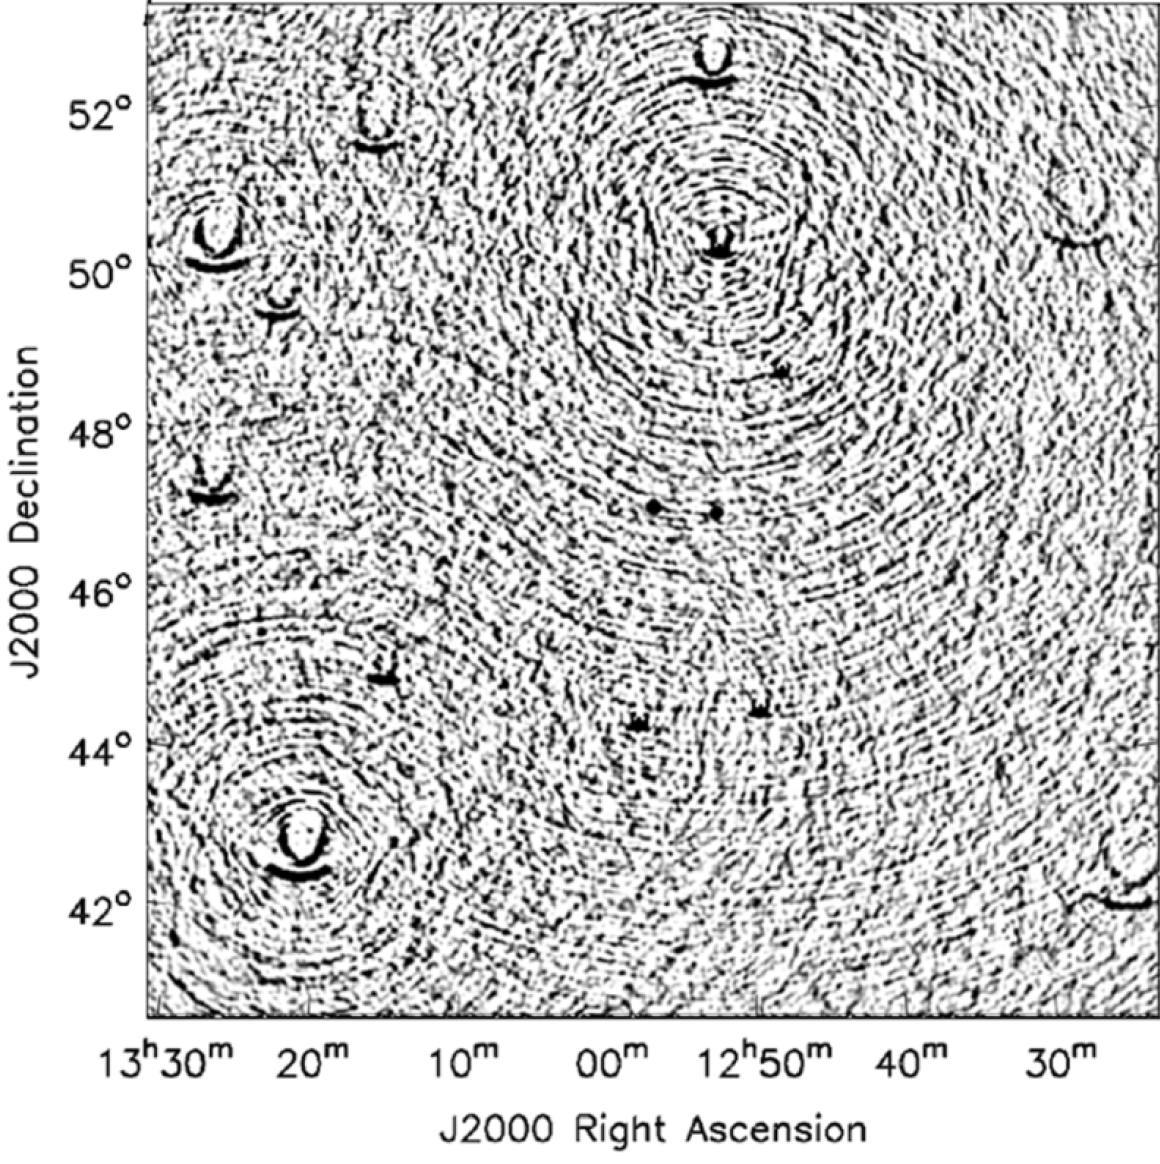
\includegraphics[width=\linewidth]{./chapters/03.radio/w-no-correction.png}
		\caption{Fourier Transform.}
		\label{results:g55:nrao:rec}
	\end{subfigure}
	\begin{subfigure}[b]{0.45\linewidth}
		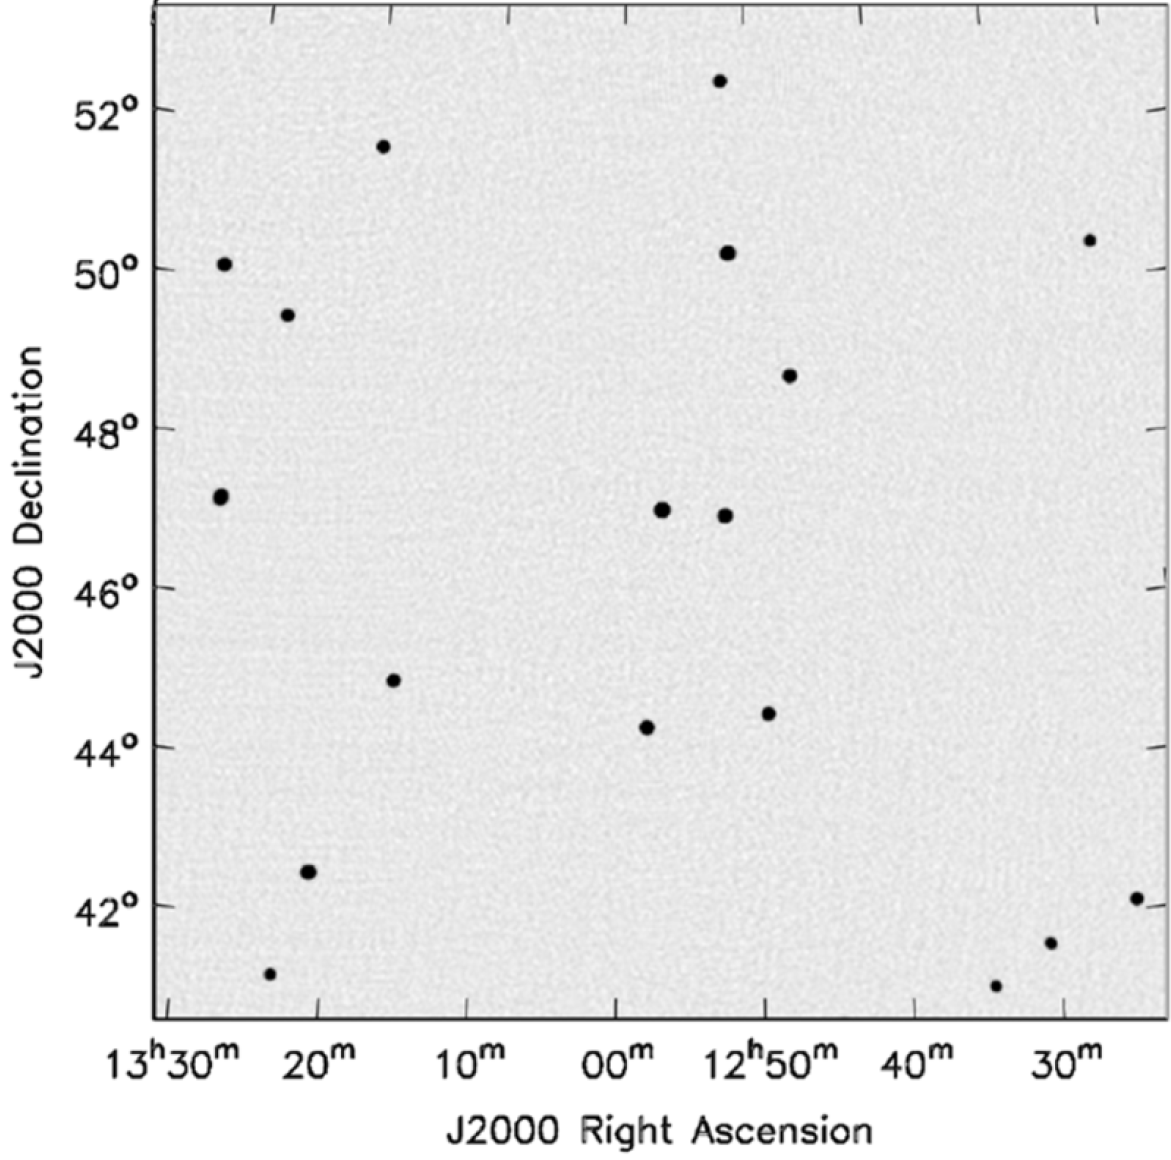
\includegraphics[width=\linewidth]{./chapters/03.radio/w-correction.png}
		\caption{Fourier Transform with w correction.}
		\label{results:g55:nrao:dirty}
	\end{subfigure}
	\caption{Effects of the w term on simulated data. Source: \cite{cornwell2008noncoplanar}}
	\label{results:g55:nrao}
\end{figure}


So far the small Field of View inverse problem has been introduced where each antenna pair measures a Visibility of the sky brightness distribution. This leads to the small Field of View measurement equation \eqref{radio:eq:2dft}. It is identical to the two dimensional Fourier Transform. In practice the Fast Fourier Transform (FFT) is used, since it scales with $~n\:log(n)$ instead of $~n^2$ pixels.



For wide Field of View imaging, two effects break the two dimensional Fourier Transform relationship: Non-coplanar Baselines and the celestial sphere which lead to the measurement equation \eqref{radio:eq:ftSphere}. Note that for small Field of View $1 - x^2 -y ^2 \ll 1$, and \eqref{radio:eq:ftSphere} reduces to the 2d measurement equation \eqref{radio:eq:2dft}.

\begin{equation}\label{meerkat:ftsphere}
	V(u, v, w) = \int\int \frac{X(x, y)}{\sqrt{1 - x^2 - y ^2}} e^{2 \pi i (ux+vy+ w\sqrt{1 - x^2 - y ^2})}dx dy
\end{equation}

\begin{wrapfigure}{r}{0.5\textwidth}
	\centering
	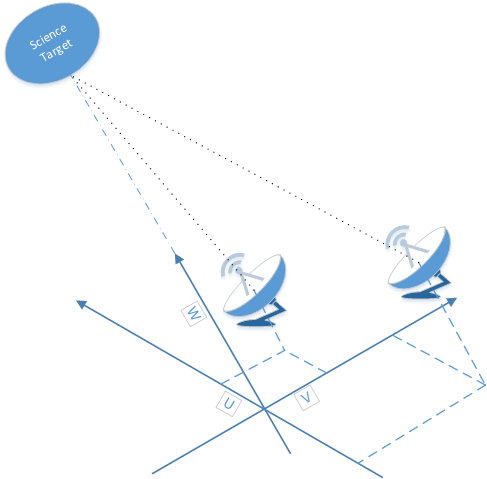
\includegraphics[width=0.9\linewidth]{./chapters/03.radio/uvw.png}
	\caption{U V and W coordinate space}
	\label{radio:uvw}
	\vspace{-10pt}
\end{wrapfigure}

Non-coplanar Baselines lead to a third component $w$ for each Visibility. Figure \ref{radio:uvw} shows the the $u$ $v$ and $w$ coordinate system. $w$ is essentially the pointing direction of the instrument. The UV-Plane is the projection of the antennas on a plane perpendicular to the pointing direction. Which point in the UV-Plane get sampled and what $w$ component it has depends on the pointing direction. If the instrument points straight up, the UV-Plane is a tangent to earth's surface, and the $w$ term compensates for earth's surface curvature. If however the instrument points at the horizon, the projected UV-Plane gets squashed and $w$ compensates for antennas which lie far behind the UV-Plane. In essence, $w$ is a phase delay that corrects antenna positions in three dimensions. The wide Field of View measurement equation \eqref{radio:eq:ftSphere} would account for the $w$ phase delay, but it breaks the the two dimensional Fourier relationship and the FFT cannot be used. The W-Projection \cite{cornwell2008noncoplanar} algorithm approximates the effect of the $w$ term restores the two dimensional Fourier relationship.


\subsection{Self-Calibration}
Why self calibration

Self calibration with clean




\subsection{State of the Art: Distributing the W-Term with WSCLEAN} 

\cite{offringa2014wsclean} WSCLEAN

Essentially distributing the non-uniform FFT of the Major Cycle.

Architecture of W-Stacking

(talking about more recent hybrid approach, limiting the total number of ?w-stacks?)







\newpage
\section{Benchmark}
\newpage
\section{results}
\newpage
\section{Conclusion}

\newpage
\bibliography{mybib}{}
%\bibliographystyle{plain}
\bibliographystyle{unsrt}
\newpage
\listoffigures
\listoftables

\newpage
\input{./chapters/99.attachment/attachment.tex}
\newpage
\section{Ehrlichkeitserklärung}
Hiermit erkläre ich, dass ich die vorliegende schriftliche Arbeit
selbstständig und nur unter Zuhilfenahme der in den Verzeichnissen oder
in den Anmerkungen genannten Quellen angefertigt habe. Ich versichere
zudem, diese Arbeit nicht bereits anderweitig als Leistungsnachweis
verwendet zu haben. Eine Überprüfung der Arbeit auf Plagiate unter
Einsatz entsprechender Software darf vorgenommen werden.\\
Windisch, \today\\[4\baselineskip]
Jonas Schwammberger 

\end{document}